% Premium TikZ pipeline figure.  Compile:  pdflatex pipeline.tex
% To embed in the paper: copy the tikzpicture into a figure environment and add
% the \usepackage / \usetikzlibrary lines (and \definecolor block) to the preamble.
\documentclass[border=14pt]{standalone}
\usepackage[scaled=0.95]{helvet}     % Helvetica (clean sans)
\renewcommand{\familydefault}{\sfdefault}
\hyphenpenalty=10000 \exhyphenpenalty=10000   % no word hyphenation in cards
\usepackage{tikz}
\usetikzlibrary{positioning, arrows.meta, backgrounds, fit, shadows.blur, calc}

\definecolor{ink}{HTML}{172029}
\definecolor{sub}{HTML}{64727F}
\definecolor{dataC}{HTML}{2D6BE4}
\definecolor{netC}{HTML}{D14D57}
\definecolor{fuseC}{HTML}{1FA06A}
\definecolor{featC}{HTML}{C99A2E}
\definecolor{embC}{HTML}{E08A3C}
\definecolor{evalC}{HTML}{7E57C2}
\definecolor{band}{HTML}{EDF1F6}

\newcommand{\stagehdr}[1]{\textbf{\color{ink}#1}}
\newcommand{\stagesub}[1]{\\[2pt]{\scriptsize\color{sub}#1}}
\newcommand{\cardhdr}[2]{{\bfseries\color{#1}#2}\\[2.5pt]%
  {\color{#1}\rule{\linewidth}{0.5pt}}\\[3pt]}

\begin{document}
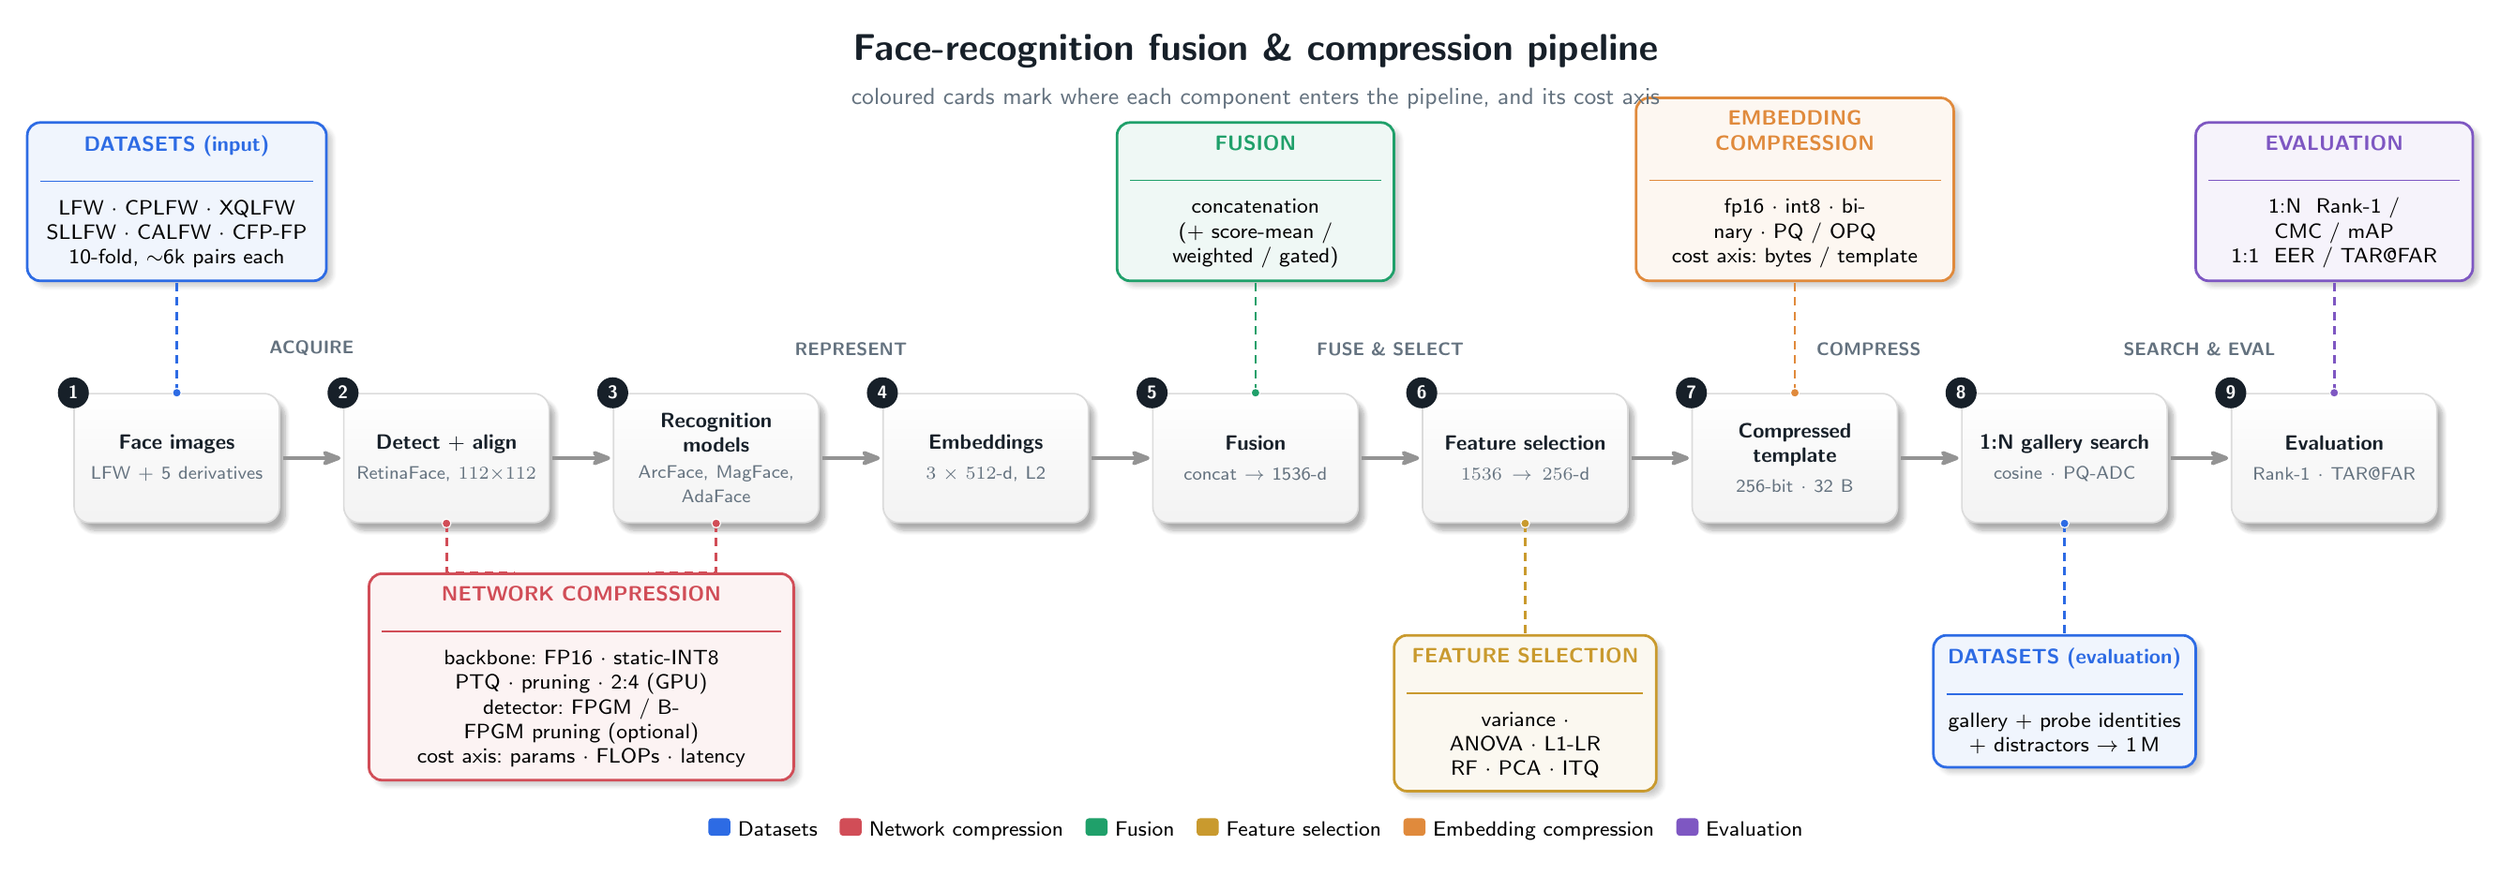
\begin{tikzpicture}[
  >={Stealth[round]},
  font=\footnotesize,
  stage/.style={rounded corners=6pt, draw=black!14, line width=0.6pt,
    top color=white, bottom color=black!5, text width=2.5cm, align=center,
    minimum height=1.75cm, inner sep=4pt,
    blur shadow={shadow blur steps=9, shadow yshift=-3pt, shadow opacity=32}},
  num/.style={circle, fill=ink, text=white, font=\bfseries\scriptsize,
    inner sep=0pt, minimum size=4.2mm},
  card/.style={rounded corners=5pt, line width=1pt, align=center, inner sep=5pt,
    blur shadow={shadow blur steps=6, shadow yshift=-2pt, shadow opacity=20}},
  arr/.style={->, line width=1.5pt, draw=black!42, shorten >=1pt, shorten <=1pt},
  conn/.style={dashed, dash pattern=on 3.2pt off 2.4pt, line width=1pt,
    line cap=butt, rounded corners=0pt},
  tap/.style={fill=#1, draw=white, line width=0.4pt},
]

% ---------- spine (9 stages) ----------
\node[stage] (s1) {\stagehdr{Face images}\stagesub{LFW $+$ 5 derivatives}};
\node[stage, right=0.85cm of s1] (s2) {\stagehdr{Detect $+$ align}\stagesub{RetinaFace, $112{\times}112$}};
\node[stage, right=0.85cm of s2] (s3) {\stagehdr{Recognition models}\stagesub{ArcFace, MagFace,\\ AdaFace}};
\node[stage, right=0.85cm of s3] (s4) {\stagehdr{Embeddings}\stagesub{$3\times512$-d, L2}};
\node[stage, right=0.85cm of s4] (s5) {\stagehdr{Fusion}\stagesub{concat $\rightarrow$ 1536-d}};
\node[stage, right=0.85cm of s5] (s6) {\stagehdr{Feature selection}\stagesub{$1536\rightarrow256$-d}};
\node[stage, right=0.85cm of s6] (s7) {\stagehdr{Compressed template}\stagesub{256-bit $\cdot$ 32 B}};
\node[stage, right=0.85cm of s7] (s8) {\stagehdr{1:N gallery search}\stagesub{cosine $\cdot$ PQ-ADC}};
\node[stage, right=0.85cm of s8] (s9) {\stagehdr{Evaluation}\stagesub{Rank-1 $\cdot$ TAR@FAR}};

\foreach \a/\b in {s1/s2,s2/s3,s3/s4,s4/s5,s5/s6,s6/s7,s7/s8,s8/s9}
  \draw[arr] (\a.east) -- (\b.west);

\foreach \s/\n in {s1/1,s2/2,s3/3,s4/4,s5/5,s6/6,s7/7,s8/8,s9/9}
  \node[num] at (\s.north west) {\n};

% ---------- phase bands (background) ----------
\begin{scope}[on background layer]
  \node[fill=band, rounded corners=11pt, fit=(s1)(s2), inner sep=9pt] (pA) {};
  \node[fill=band, rounded corners=11pt, fit=(s3)(s4), inner sep=9pt] (pB) {};
  \node[fill=band, rounded corners=11pt, fit=(s5)(s6), inner sep=9pt] (pC) {};
  \node[fill=band, rounded corners=11pt, fit=(s7),      inner sep=9pt] (pD) {};
  \node[fill=band, rounded corners=11pt, fit=(s8)(s9), inner sep=9pt] (pE) {};
\end{scope}
\foreach \p/\t in {pA/ACQUIRE, pB/REPRESENT, pC/FUSE \& SELECT, pE/SEARCH \& EVAL}
  \node[above=1.5pt of \p.north, font=\bfseries\scriptsize, color=sub] {\t};
% COMPRESS shifted clear of stage-7's straight connector column
\node[above=1.5pt of pD.north, xshift=1.0cm, font=\bfseries\scriptsize, color=sub] {COMPRESS};

% ---------- annotation cards ----------
\node[card, draw=dataC, fill=dataC!7, text width=3.7cm, above=1.5cm of s1] (cIn)
  {\cardhdr{dataC}{DATASETS (input)} LFW $\cdot$ CPLFW $\cdot$ XQLFW\\ SLLFW $\cdot$ CALFW $\cdot$ CFP-FP\\ 10-fold, $\sim$6k pairs each};

\coordinate (mNet) at ($(s2)!0.5!(s3)$);
\node[card, draw=netC, fill=netC!7, text width=5.4cm, below=1.55cm of mNet] (cNet)
  {\cardhdr{netC}{NETWORK COMPRESSION}
   backbone:\ FP16 $\cdot$ static-INT8 PTQ $\cdot$ pruning $\cdot$ 2:4 (GPU)\\
   detector:\ FPGM / B-FPGM pruning (optional)\\
   cost axis:\ params $\cdot$ FLOPs $\cdot$ latency};

\node[card, draw=fuseC, fill=fuseC!7, text width=3.4cm, above=1.5cm of s5] (cFus)
  {\cardhdr{fuseC}{FUSION} concatenation\\ ($+$ score-mean / weighted / gated)};

\node[card, draw=featC, fill=featC!7, text width=3.2cm, below=1.5cm of s6] (cFeat)
  {\cardhdr{featC}{FEATURE SELECTION} variance $\cdot$ ANOVA $\cdot$ L1-LR\\ RF $\cdot$ PCA $\cdot$ ITQ};

\node[card, draw=embC, fill=embC!7, text width=3.95cm, above=1.5cm of s7] (cEmb)
  {\cardhdr{embC}{EMBEDDING COMPRESSION} fp16 $\cdot$ int8 $\cdot$ binary $\cdot$ PQ / OPQ\\ cost axis:\ bytes / template};

\node[card, draw=dataC, fill=dataC!7, text width=3.2cm, below=1.5cm of s8] (cEval)
  {\cardhdr{dataC}{DATASETS (evaluation)} gallery $+$ probe identities\\ $+$ distractors $\rightarrow$ 1\,M};

\node[card, draw=evalC, fill=evalC!7, text width=3.4cm, above=1.5cm of s9] (cMet)
  {\cardhdr{evalC}{EVALUATION} 1:N\ \ Rank-1 / CMC / mAP\\ 1:1\ \ EER / TAR@FAR};

% ---------- connectors: STRAIGHT where the card sits over its stage; orthogonal otherwise ----------
\draw[conn, dataC] (s1.north) -- (cIn.south);
\draw[conn, fuseC] (s5.north) -- (cFus.south);
\draw[conn, embC]  (s7.north) -- (cEmb.south);
\draw[conn, evalC] (s9.north) -- (cMet.south);
\draw[conn, featC] (s6.south) -- (cFeat.north);
\draw[conn, dataC] (s8.south) -- (cEval.north);
% only the network card straddles two stages -> sharp orthogonal "edgy" routing
\draw[conn, netC]  (s2.south) |- ($(cNet.north)+(-0.9,0)$);
\draw[conn, netC]  (s3.south) |- ($(cNet.north)+(0.9,0)$);
\foreach \c/\s/\d in {dataC/s1/north, fuseC/s5/north, embC/s7/north, evalC/s9/north,
  featC/s6/south, dataC/s8/south, netC/s2/south, netC/s3/south}
  \filldraw[fill=\c, draw=white, line width=0.4pt] (\s.\d) circle (1.7pt);

% ---------- title + legend ----------
\node[text=ink, font=\Large\bfseries] (ttl) at ($(s5 |- cIn.north)+(0,0.95)$)
  {Face-recognition fusion \& compression pipeline};
\node[below=1pt of ttl, text=sub, font=\small]
  {coloured cards mark where each component enters the pipeline, and its cost axis};

\node[anchor=north, font=\footnotesize] (leg) at ($(s5 |- cEval.south)+(0,-0.55)$) {%
  \tikz[baseline]{\fill[dataC,rounded corners=1.4pt](0,0)rectangle(0.30,0.24);}~Datasets\quad
  \tikz[baseline]{\fill[netC,rounded corners=1.4pt](0,0)rectangle(0.30,0.24);}~Network compression\quad
  \tikz[baseline]{\fill[fuseC,rounded corners=1.4pt](0,0)rectangle(0.30,0.24);}~Fusion\quad
  \tikz[baseline]{\fill[featC,rounded corners=1.4pt](0,0)rectangle(0.30,0.24);}~Feature selection\quad
  \tikz[baseline]{\fill[embC,rounded corners=1.4pt](0,0)rectangle(0.30,0.24);}~Embedding compression\quad
  \tikz[baseline]{\fill[evalC,rounded corners=1.4pt](0,0)rectangle(0.30,0.24);}~Evaluation};

\end{tikzpicture}
\end{document}
